\documentclass[a4paper]{paper} 
%\usepackage{babel}
\usepackage{hyperref}
\usepackage{amsfonts}
\usepackage{amsmath}
\usepackage{graphicx}
\usepackage[space]{grffile}
\usepackage[margin=2.5cm]{geometry}
\usepackage{pdfpages}
%\usepackage{graphicx}
\usepackage[capitalize,noabbrev]{cleveref}

\DeclareMathOperator*{\argmax}{arg\,max}

\graphicspath{{img/}}
\title{Network balance improvement algorithm for payment networks}
\subtitle{Draft version}
\author{Rene Pickhardt and Mariusz Nowostawski} 
\institution{NTNU Gj{\o}vik} 

\begin{document} 
\twocolumn[\maketitle 
\hrule 
\begin{abstract}
Making a payment in privacy aware payment channel networks is currently achieved by trying several payment paths until one succeeds which can yield to several minutes for a payment to complete.
We introduce a network imbalance measure and formulate the optimization problem of improving the balance of the network as a sequence of rebalancing operations of the funds within the channels along circular paths within the network.
As the funds and balances of channels are not globally known we introduce a greedy heuristic with which every node despite the uncertainty can improve its own local balance.
In an empirical evaluation on a recent snapshot of the Lightning Network we show that the imbalance distribution of the network has a Kolmogorov Smirnoff distance of $0.74$ in comparison to the imbalance distribution after the heuristic is applied.
We further show that the success rate of a tiny payment increases from $11.2\%$ on the imbalanced network to $98.3\%$ in the balanced network.
 Similarly the median possible payment size accross all pairs of participants increases from $0$ to $0.5$ mBTC for initial routing attempts on the cheapest possible path.
We provide emperical and game theoretic evidence that routing fees should be dropped for proactive rebalancing operations.
Executing $4$ different strategies for selecting rebalancing cycles lead to similar results indicating that a collaborative approach within the friend of the friend network might be preferable from a practical point of view.

\end{abstract}

\begin{keywords}
Imbalance, rebalancing, Optimization, Bitcoin, Lightning Network, payment channel networks, path finding, routing, liquidity, flow control, congestion control, game theory, uncertainty, simulations, agent based systems, collaborative problem solving, privacy 
\end{keywords}
\hrule\bigskip
]


%==========================================================================
\section{Introduction}
Payment channel networks have been introduced in order to mitigate the scaling issues of blockchain technologies such as Bitcoin\cite{poon2016bitcoin}.
With the help of smart contracts payment channels are created that allow the cryptographically secure transfer of value without the necessity to record the transaction to the central ledger.
This yields new and interesting privacy properties for the participants of the network.
In order to protect the privacy while routing a payment through several payment channels privacy aware payment channel networks use a source based onion routing scheme like the Sphinx Mix format \cite{danezis2009sphinx}.
This prevents routing nodes from learning who paid whom.

While the lightning network for example shares the capacity of public channels with its participants through its gossip protocol the local split of the capacity of the channels into the balance of its participants is not being shared with the rest of the network for two reasons:
First this would compromise the privacy as one could collect all changes of the channel balances and reconstruct the flow of payments.
Second propagating this information would essentially mean that every node in the network is made aware of every payment which would have the same poor scaling properties as blockchain technologies and other broadcast networks.
The decision to use source base routing together with the unknown channel balances of the network results in a challenge for finding a path of payment channels so that all channels along the path have enough liquidity to be able to forward an attempted payment.
Currently this challenge is met by probing paths with a brute force approach until one such path is found.
It has been shown that probing for paths can take more than 3 minutes for more than $5\%$ of the attempted payments \cite{decker2019lnconf} which leads to a poor user experience.
Imagine a grocery store in which for every $20^{th}$ customer the cash register would have to wait three minutes until the payment was received.

In this paper we examine the consequences of nodes proactively and collaboratively distributing their funds evenly across their channels.
We introduce the notation of an imbalanced network.
The imbalance is measured as the average of the imbalance scores of its nodes.
The node's imbalance of payment channels i defined as the gini coefficient of a node's channel balance coefficients which are the relative amount of funds a node owns in a channel in comparison to the capacity of that channel.
In particular nodes already have all the information they need to compute their imbalance. 
Nodes can reduce their imbalance either alone or collaboratively with the help of their channel partners by conducting circular payments which is also known as rebalancing.
Another option is by using a submarine swap\footnote{\url{https://github.com/submarineswaps/swaps-service}} as an off-chain / on-chain swapping service.

We formulate an optimization problem of finding a sequence of rebalance operation that minimizes the network's imbalance.
As the information necessary to solve the optimization problem is not publically known in privacy aware payment channel networks we provide a greedy privacy aware agent based heuristic for its participants to find a minimum for the problem. 
In an empirical study we show that the greedy heuristic will lead to a success rate of $98.3\%$ for a small payment between two arbitrary selected nodes.
Also the median possible payment size between all pairs of nodes increases from $0$ in the imbalanced network to $0.5$ mBTC in the best balanced networks that we found.

While single nodes can already execute the algorithm in currently existing payment channel networks they have to pay routing fees for rebalancing operations.
Thus economically they are disincentivized to do so.
We compared the earned fees for being participant of another nodes rebalancing attempt and the paid fees for initiating rebalancing operations.
Showing that these numbers are normally distributed around $0$ we propose to omit fees for proactive rebalancing operations to incentivice nodes to execute our algorithm which seems to be benefitial for the entire network. 
Looking at different strategies of finding rebalancing cycles that the algorithm uses we suggest for the sake of speed that nodes share with their neighbors on which local channels they would like to have inbound or outbound capacity.
This information could easily be probed anyway and seems not to worsen the privacy of nodes.

The remainder of this paper is organized as follows: In section \cref{sec:relatedWork} we give a short overview of related work in this field.
We then introduce the notation and definition of the imbalance score in section \cref{sec:formalization} and formulate the optimization problem to reduce the imbalance.
We propose a greedy, agent based and collaborative algorithm in \ref{sec:Algorithm} to address the optimization problem.
We also propose different strategies for the algorithm to probe for potential rebalancing cycles.
In \cref{sec:setup} we introduce the experimental setup and the data set that we used.
After showing our empirical results in \cref{sec:results} we discuss the results and propose some future work in the last two sections.



%==========================================================================
\section{Related Work}
\label{sec:relatedWork}

While the Lightning Network White paper~\cite{poon2016bitcoin} does not discuss path finding and states routing as an easy problem it is generally recognized that pathfinding on the lightning network is a difficult problem \cite{piatkivskyi2018split, prihodko2016flare, bagaria2019boomerang, pickhardt2019pathfinding, grunspan2018ant, sivaraman2018routing}.
There is already research being conducted in the field of rebalancing channels~\cite{khalil2017revive} which was more about the cryptographic protocols used to make sure that participants can enforcethe rebalancing that was agreed upon.
There are rebalancing operations for c-lightning\footnote{\url{https://github.com/lightningd/plugins/tree/master/rebalance}} and for lnd\footnote{\url{https://github.com/bitromortac/lndmanage}}.
In particular the idea of Just in time rebalancing while fulfilling routing requests~\cite{pickhardt2019jit} is already being implemented as JIT-routing for c-lightning\footnote{\url{https://github.com/lightningd/plugins/pull/66}}. 

% ===========================================================================
\section{Formalization and Assumptions}
\label{sec:formalization}

Let $G=(V,E,c)$ be a privacy aware payment channel network with a finit set of nodes.
The payment channels are the edges in the network such that $E\subset V\times V$.
Additionally we have a publicly known capacity function $c: E\longrightarrow \mathbb{N}$ that assigns a capacity to every edge of the network.
For every edge $e=(u,v)$ we denote $e_u:=(e,u)$ as the first participant of the channel and $e_v=(e,v)$ as the second participant.
Every node can be assigned its set of channels which we encode with the neighbor function $n : V \longrightarrow 2^{E}$.
Similarly, if we want to denote the set of neighboring nodes we use the function $n_n : V \longrightarrow 2^{V}$.
Naturally, the capacity of every channel $e=(u,v)$ is privately split into the local balances with the balance function $b: E\times N\longrightarrow\mathbb{N}$ such that $b(e_u)+b(e_v)\stackrel{!}{=}c(e)$.

We define the channel balance coefficient for $u$ on the channel $e=(u,v)$ as  $\zeta_{(u,v)} = \frac{b(e_u)}{c(e)}$.
This is just the relative amount of funds that the participant $u$ has in the channel $e$.
Note since $b(e_u)+b(e_v)\stackrel{!}{=}c(e)$ we also have $\zeta_{(u,v)} + \zeta_{(v,u)}=1$.
in particular we have $\zeta_{(u,v)} \neq \zeta_{(v,u)}$ 

The total funds of a participant $u$ are denoted as $\tau_u:=\displaystyle{\sum_{e\in n(u)}b(e_u)}$.
The value of $\tau_u$ is constant while no payments are made and no channels are being opened and closed.
In contrast the balance function $b$ can vary subject to re-allocation of funds.
To make the following formulas easier to read let us introduce $U:=n(u)$ which denotes the set of channels which participant $u$ is part of.
The total capacity of a participant $u$ is denoted as $\kappa_u:=\displaystyle{\sum_{e\in U}c(e)}$.
Using the last two definitions let us define the node balance coefficient for a participant $u$ as $\nu_u = \frac{\tau_u}{\kappa_u}$.

We call a node $u$ {\bf balanced} if its channel balance coefficients $\zeta_{(u,v_1)},\dots,\zeta_{(u,v_d)}$ have the same value.
This means that the distribution of a node's relative funds across all its channels is the same.
Consequently, we consider a node {\bf unbalanced}, if it local channel balance coefficients are unequal.
Statistically, inequality of a distribution can be measured with the Gini coefficient.
Thus, for a node $u$ with channel balance coefficients $\zeta_{(u,v_1)},\dots,\zeta_{(u,v_d)}$ we define $G_u = \frac{\displaystyle{\sum_{i\in U} \sum_{j \in U}} | \zeta_i - \zeta_j |}{2 \displaystyle{\sum_{i \in U} \sum_{j \in U} \zeta_j}}$
If $G_u = 0$ this means that the channel balance coefficents are equal.
In contrast, if $G_u = 1$ the channel balance coefficients are distributed in the most unequal way.

Note, that the Gini coefficient of a channel balance coefficients of a node $u$ takes the value $0$ if and only if its channel balance coefficents all take the same value.
This value will be exactly the same as the node's balance coefficient $\nu_u$.
Nodes which have channels with large differences in capacities will not be able to get a Gini coefficient of 0 if we used absolute balances for the definition of the $\zeta$ values as in such cases smaller channels might be drained by larger ones during rebalancing operations.

Finally, $G$ denotes the imbalance of the network. $G = \displaystyle{\frac{1}{|N|}\sum_{n\in N}G_n}$. It is the mean of the imbalance values of all nodes in the network.
A perfectly balanced network would be achieved if $G$ takes the value of $0$ whereas the balance is poor if the value of $G$ is close to 1.

Our goal is to find a balance function $b$ which minimizes $G$ given a privacy aware payment channel network with initial distribution of funds $\tau_{u_1},\dots,\tau_{u_n}$.
The constraint to this optimization problem is that the total funds $\tau_u$ are fixed for every node $u \in N$ and any choice of the balance function $b$.
In a privacy aware payment channel network the distribution of funds $\tau_{u_1}\dots,\tau_{u_n}$ is not publicly known.\footnote{The initial distribution could be guessed from the funding transactions in the case of the Bitcoin Lightning Network for public channels. Note, this distribution will change with the first payment that is not a rebalancing operation.}
In the same way the initial balance function is not publicly known.
As we lack knowledge about the global network state, we cannot apply standard optimization techniques such as gradient descent, conjugate gradient methods or simulated annealing.
We suggest to use an agent based heuristic in which every participant executes some operations to improve its own balance which others support if it also improves their balance.

\subsection{Description of the rebalancing algorithm}
\label{sec:Algorithm}

The algorithm solves the optimization problem of finding $b$ such that the balance of the network is improved.
The developed rebalancing algorithm uses an agent-based heuristic in which participants use the local knowledge and make local adjustments. 
This results in a global convergence towards an improved overall network balance. 

\begin{enumerate}
\item A node $u$ will compute its node balance coefficient $\nu_u$.
\item $u$ will then compute the channel balance coefficients $\zeta_{(u,v_1)},\dots,\zeta_{(u,v_d)}$ for its $d$ channels.
\item The node will select all channels $e=(u,v_i)$ for which its channel balance coefficient is higher 
than its node balance coefficient, i.e.~$C = \{(u,v_i) | \zeta_{(u,v_i)} - \nu_u\ > 0\}$\footnote{
  Note, that we do not need to take absolute values as $u$ will only be able to initiate a rebalancing operation by sending money which means decreasing its channel balance coefficient of $\zeta_{(u,v_i)}$.}.
\item from the candidate set $C$ a random channel $e=(u,v)$ is selected.\footnote{
  We show in the experimental evaluation that always taking the channel with the biggest gain makes the heuristic stuck too quickly. 
  The reason is that if a channel cannot be rebalanced in the next step the same channel is tried again.} 
\item Now the node searches for a circular payment to itself along $e=(u,v)$ within its friend of a friend network by choosing a path $p = [u,v,x_1,\dots,x_n,u]$. The amount of that payment should decrease the value of $\zeta_{(u,v)}$ to that of $\nu_u$ and can be computed as $a = c(e)\cdot (\zeta_{(u,v)}-\nu_u)$. The end of the circle should be a channel $(x_n,u)$ for which the channel balance coefficient $\zeta_{(u,x_n)}$ is smaller than the node balance coefficient $\nu_u$.\footnote{In one of the experiments we weaken this strong critera and show emperically that it makes sense to drop it.}
\item The node conducts the payment if all the nodes on the path $p$ agree to participate. 
\item Repeat all steps as long as the local balance coefficients are not even enough.
\end{enumerate}

When a circular path exists, it is easy to see that making a payment along this path will make the distribution of local balance coefficients for node $u$ more even.
If no such circular path can be found the local balance stays constant.
Finding a circular rebalancing path might be difficult as the balances within the network are not known. 
However, this problem is not worse than the current problem of probing paths for regular payments.

\section{Experimental Setup}
\label{sec:setup}

We conducted our experiment on a snapshot of the public Lightning Network from October 2019.
That network view was retrieved from the gossip store of our lightning node which is accassible at \url{https://ln.rene-pickhardt.de}.
The distribution of funds in the Lightning Network is not a public information and had to be guessd in the following way.
As channels are currently almost always opened by one side\footnote{Dual funded channels are not part of the protocol and no implemention is merged to any of the standard nodes} we randomly guessed who opened the channel by a coinflip and allocated the entire channel capacity to the node that was chosen by the coinflip. 
This had to be done as the gossip protocol also does not propagate any information about who is opening the protocol.
\begin{figure}
 \centering
 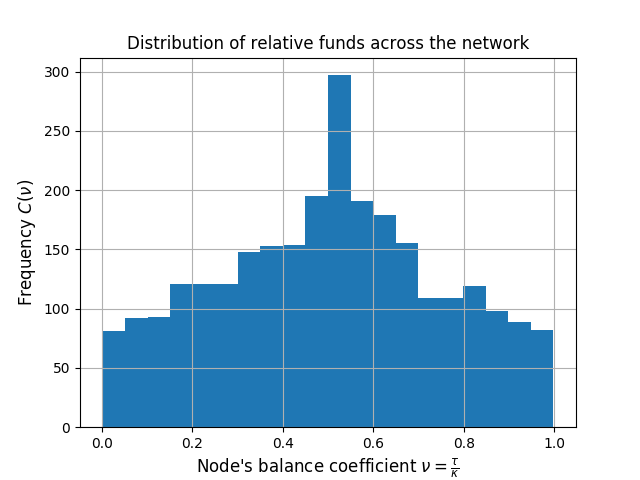
\includegraphics[width=8cm]{code/vs/fig/distribution_of_nus.png}
 \caption{The histogram shows the distribution of relative funds $\nu_v$ for each node $v\in G$.}
 \label{fig:initial_funds}
\end{figure}
From figure \cref{fig:initial_funds} we can see the result of our random process of allocating funds to the nodes.

After we randomly chose the funder of each channel we computed the largest strongly connected component.
This mainly removed nodes which only have one channel or due to our random process had opened all channels or have been receiving all channels from others.
all of these nodes could not take place in any rebalancing operation anyway.
The strongly connected component consists of $2707$ nodes and $24161$ edges.
The diameter of the strongly connected component had a value of 10 and the cumulative distance distribution of shortest paths between all pairs can be seen in figure \cref{fig:cumulative_distance}
\begin{figure}
 \centering
 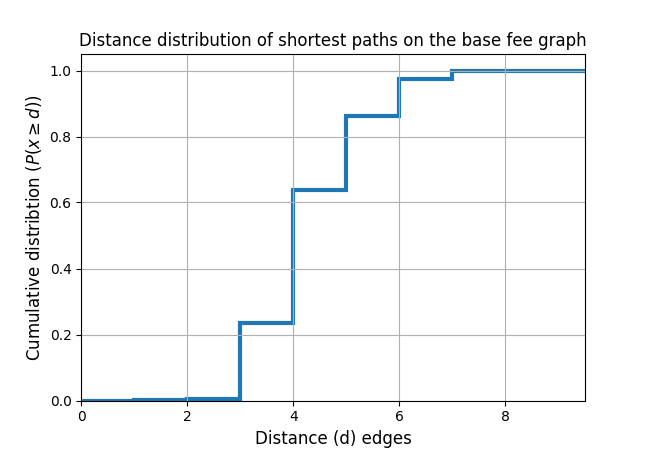
\includegraphics[width=8cm]{code/vs/fig/cummulative_distance_distribution_lin_scale.png}
 \caption{Probability mass of pathlengths of shortest paths between all pairs of nodes. As this is computed on the strongly connected component there will always be a path between each pair of nodes}
 \label{fig:cumulative_distance}
\end{figure}
Note that the notion of shortest paths with respect to fees is depending on the amount that is being transfered as the fees on channels have a fixed base fee and a variable fee rate.
For the computation of shortest paths we have assumed a fixed payment size and essentially computed the shortest paths by only respecting the fixed base fee.

It is interesting to note that about $40\%$ of pahts have 5 or more hops.
This means that a shortest rebalancing cycle would have at least 6 hops.
This demonstrates that the single rebalancing operations which we conducted where no covering the entire network but only taking place within local parts of the network.
This is particularly true for the rebalancing in the friend of a friend network.

\begin{figure}
 \centering
 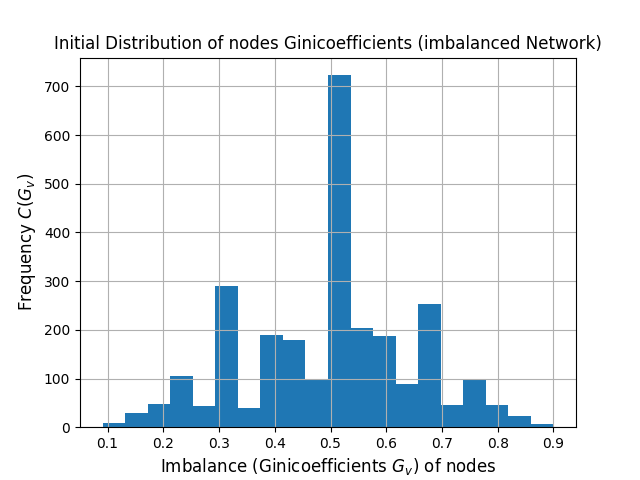
\includegraphics[width=8cm]{code/vs/fig/initial_ginis_before_rebalancing.png}
 \caption{The distribution of Gini coefficients for each node over its distribution of channel balance coefficients $\zeta$ of the input network before any rebalancing experiment was taking place.}
 \label{fig:initial_ginis}
\end{figure}
Figure \cref{fig:initial_ginis} depicts the initial distribution of Ginicoefficients for each node of the examined network.
This plot also reflects the random nature of the allocated funds already resulting in an average value as the total network imbalance very close to $0.5$.

In order to conduct the experiments we simulated the proposed algorithm and strategies in the following way.
For each channel we computed up to 5000 rebalancing cycles which included this channel.
These cycles followed the properties defined by the strategy (for example fixing the maximal length).
The number $5000$ was chosen to be as large as possible so that we where able to conduct the simulation within the $16$ GB of main memory of our machine.
In most cases \footnote{we didn't count them} there where less than $5000$ cycles available.
However sometimes we had to cut off the precomputed cycles as the hard cap of $5000$ was hit.

For each cycle we checked if a rebalancing was possible without having nodes on the path worsening their channel balance coefficients.
As this assumption is very strong the vast majority in rebalancing attempts along a cycle would fail or only work with an amount smaller than the one proposed by the initiator. 
In particular for the multipath payments we did not rebalance the entire possible amount but just a $20^{th}$ of it.
Also we allowed in the foaf rebalancing and multipath rebalancing that the node who initiated the rebalancing could also worsen the situation for its final channel.\footnote{This effectively means that we did not have to compute all cycles in the foaf network but where able to build symmetric differences of a cycle base.}
This also explains why the final results for these two strategies are not entirely monotonic but oscillating a bit.

\textbf{REWRITE? MOVE TO DISCUSSION?} Computing the rebalancing circles is the most expensive operation, due to the fact that it requires solving the shortest path problem.
If the greedy heuristic is implemented in a real payment channel network this is not too expensive for a node as the shortest paths only need to be computed in a subset of the friend of a friend network.
This is typically small enough to have substantial performance overheads. 
In a real payment channel network this computation would only have to be conducted 
if the distribution of channel balance coefficients becomes too uneven,
which is easily monitored after every payment or routing attempt without performance overhead.
However, in the simulation the path finding operations limit the experiments to rather small tests and also prevents us from conducting experiments on simulated large scale payment channel networks with millions of nodes / channels.

 
% ==========================================================
\section{Results}
\label{sec:results}

\begin{figure}
 \centering
 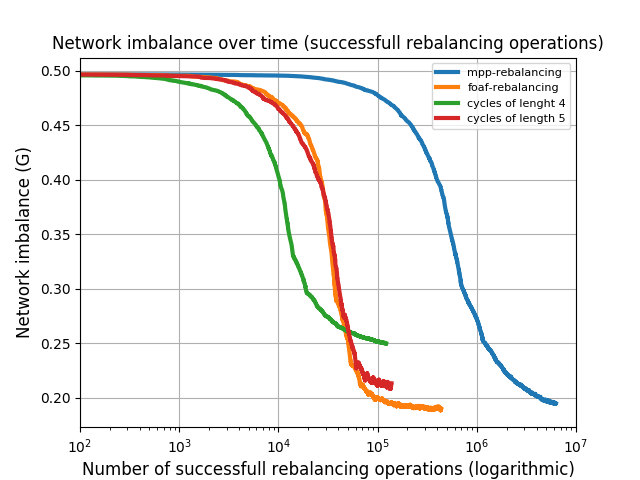
\includegraphics[width=7cm]{code/vs/fig/imba_vs_steps.png}
 \caption{Comparing how the imbalance score of the network behaves with the amount of successfull rebalancing operations. As the rebalancing amounts are much smaller with multi path payments the x-axis has a logarithmic scale.}
 \label{fig:imbalancehovertime}
\end{figure}

\cref{fig:imbalancehovertime} confirms that the balance score of the network is decreasing over time when running our simulation.
This means that the network is becoming more balanced.
We see that most improvement is happening quite fast with $10$k to $100$k rebalancing being necessary.
This is not more than $37$ rebalancing operations per node.
Taking into account that the average node degree is $9$ this means that each node needs up to $4$ rebalancing operations per channel.  
This seams plausible in the sense that every channel gets rebalanced at least once.\footnote{Note, that due to the collaborative behaviour of nodes a node also gets channel rebalanced in the rebalancing attempts of other nodes.}
The only difference is the multipath rebalancing.
This makes actully a lot of sense as we only rebalanced for a $20^{th}$ of the possible amount in the multipath case since we wanted to have multiple other paths to rebalance that particular channel.
In particular the algorithm converges in a local minimum rather quickly.
Note, that the established minimum is a local minimum. 
Our experimental runs resulted in states that are not identical when we shuffled the order of cycles that we probed, however, the differences were negligible. 
We can therefore assume that the local minimum might be close to global minimum as the collected data demonstrate.

\begin{figure}
 \centering
 
\includegraphics[width=8cm]{code/vs/fig/imba_vs_success_rates.png}
 \caption{Every time the network helth reached a new low to a two digit decimal we computed the probability for a random payment of the smallest possible amount to fail on the cheapest path.}
 \label{fig:imba_vs_success}
\end{figure}

In \cref{fig:imba_vs_success} we compare the imbalance score with the success rate of payments.
We can see that better balance scores (lower imbalance score $G$) yield a higher success rate for payments as expected.
The success rate is measured by attempting a payment between all pairs of nodes and counting the relative amount of payments that routed successfully on the cheapest path from the source to the destination through the network.
We computed the success rate of every time the balance score hits a new score rounded to two decimals.
This result confirms the dependency of the payment failure and the worse balance indicator. It is the first experiment that indicates that the defined imbalance score is semantically correct and well chosen. 
Again the multipath payment strategy sticks out as it achieves a rather high success rate while the network is still rather imbalanced.
However this is a little bit missleading for the following reasons.
A successrate of $80\%$ is reached for an imbalance score of $0.43$.
Comparing this back with figure \cref{fig:imbalancehovertime} we see that about $250$k rebalance operations are necessary to achieve this success rate.
Even the worst performing algorithm achieves this success rate with far less than $100$k rebalancing operations and a much better overall imbalance score. 

This effect - while expected as multipath rebalancing uses smaller amounts -sssssss becomes more visible in the next experiment. 
The goal of the next experiment is to check if the overall amounts that can be routed increase with better balance scores (lower imbalance metric $G$).

\begin{figure}
 \centering
 
\includegraphics[width=8cm]{code/vs/fig/imba_vs_median_payment_size.png}
 \caption{The imbalance of the network is plotted against the median value of payments that can be fulfilled betwen all pairs of nodes on the first attempt along the cheapest path. Note that failed payments are part of the statistics and counted as payments which can send $0$ satoshi.}
 \label{fig:imba_vs_payment_size}
\end{figure}

In \cref{fig:imba_vs_payment_size} we compare the imbalance of the network with the median payment amount.
The median payment amount is computed as follows.
First all pair of shortest paths (on the base fee graph) are computed.
We then look at the amount that could actually be forwarded through each path.
Finally we take the median of those amounts.
This means that at least $50\%$ of payment pairs are able to forward this amount.
The higher this amount is the higher arbitrary payments are supported by the network.
Again we see that the more balanced the network is (lower imbalance score) the higher the median payment size.
This suggests that a more balanced network is statistically able to route higher payment amounts on the first try.
This is particularly important as privacy aware payment channel networks use source based onion routing and technically have to guess a path.
When those initially guessed paths provide a high rate with high payment amounts there are considerable benefits for the overall functioning of the payment channel network. 
The user experience is improved, the payment delays are lowered, and the amount of messaging and coordination is minimised.

We note that the rebalancing along cycles in which each hop has to improve the $\zeta$ values of each participants (cycles of length $4$ and $5$) are monotonic in this diagram.
Strategies that allow cycls in which the last hop worsens the $\zeta$ value of the node who initiates the rebalancing are not monotonic.
This is the case for our implementation of multipath payments and friend of a friend rebalancing.
One can also see that mpp is not behaving best with respect to the median payment size.
In particular this becomes obvious when we remember that way more rebalancing operations have been necessary in the multipath rebalancing case.

\begin{figure}
 \centering
 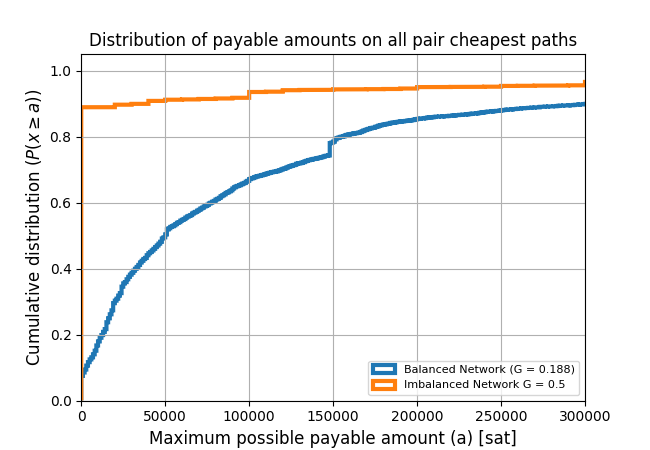
\includegraphics[width=8cm]{code/vs/fig/maximum_payable_amount_all_pair_chepest_paths_balanced_network.png}
 \caption{The maximal payable amounts on all pairs of cheapest paths on the initial imbalanced network and on the network after applying the friend of a friend rebalancing strategy.}
 \label{fig:cdf_paymentsize}
\end{figure}
We look a little bit close at the datapoint of the most balanced network with the friend of a friend strategy and compare it to the imbalanced network in figure \cref{fig:cdf_paymentsize}.
On the cumulative distribution function we can see that in the imbalanced network almost $90\%$ of the paths are not able to forward a single satoshi.
This number drops below $10\%$ for the balanced network.
The median of the balanced network takes a value of $50000$ satoshi ($0.5$ mBTC) which at the time of writing is worth about $3$ USD.
This shows that in a balanced lightning network $50\%$ of payment pairs are able to make micro payments of up to $3$ USD on the first attempt. 


For the friend of friend network we have also plotted the final distribution of Gini coefficients in figure \cref{fig:final_gini}. 
\begin{figure}
 \centering
 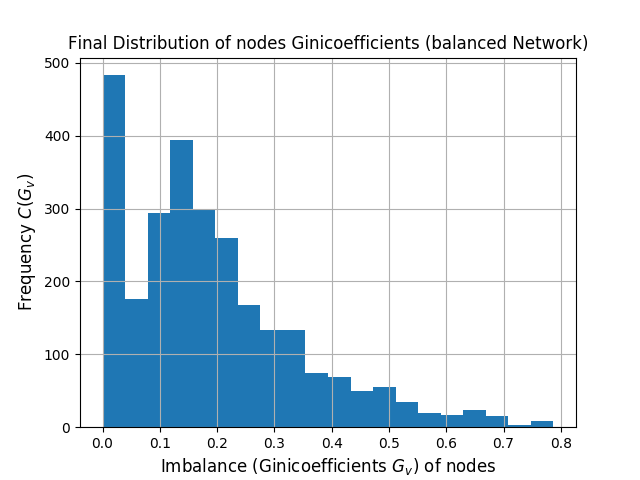
\includegraphics[width=8cm]{code/vs/fig/Final_ginis_after_rebalancing.png}
 \caption{The distribution of Gini coefficients for each node over its distribution of channel balance coefficients $\zeta$ of the network after aplying the foaf rebalancing strategy.}
 \label{fig:final_gini}
\end{figure}
As the comparison with figure \cref{fig:initial_ginis} is a little bit tricky we provide the cumulative distribution function of both distributions with a smaller bin size in figure \cref{fig:cdf_gini}

\begin{figure}
 \centering
 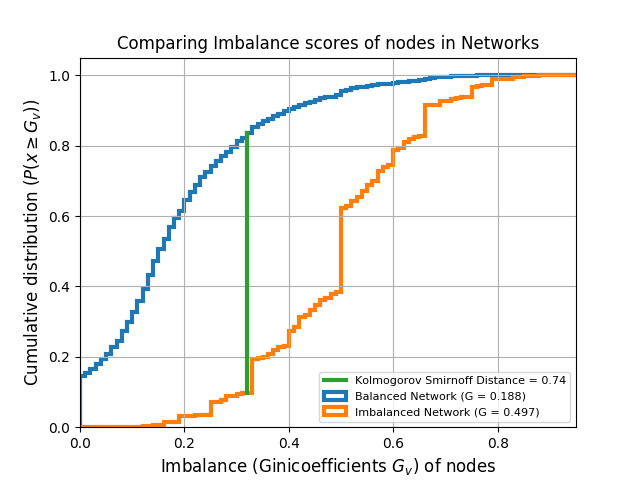
\includegraphics[width=8cm]{code/vs/fig/comparison distribution of Ginicoefficients.png}
 \caption{Coparing the distribution of the node's Gini coefficients before and afte rebalancing with the friend of a friend strategy.}
 \label{fig:cdf_gini}
 \end{figure}
 The Kolmogorov Smirnoff distance which is defined as the maximum pointwise difference of the cumulative distribution functions takes a value of $0.74$.
 This shows the statistical significance of the rebalancing heuristic in comparison to staying with the imbalanced network..
 We can see that the median value of the Ginicoefficients in the best balanced network that we could aquire is about $0.15$.
 In comparison on the imbalanced network the median Gini coefficient takes the value of $0.5$.

 As a last experiment we tracked the routing fees that nodes would have to pay for their rebalancing operations and that the would earn while they are participating in the rebalancing operation of other nodes.
 \begin{figure}
 \centering
 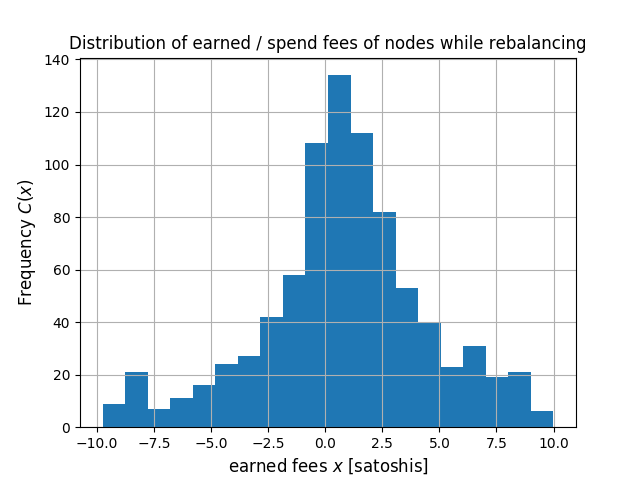
\includegraphics[width=8cm]{code/vs/fig/distribution_of_fees.png}
 \caption{Coparing the distribution of the node's Gini coefficients before and afte rebalancing with the friend of a friend strategy. Negative fees mean that the node paid more fees than it earned}
 \label{fig:fees}
 \end{figure}
 Figure \cref{fig:fees} shows that the overall fees are normally distributed around $0$.
 This means that the expected value of fees that need to be paid or are being earned if all nodes participate in proactive rebalancing is $0$.
An expected value of $0$ is a strong indicator that fees should not play a role for rebalancing operations if those are beneficial for every node that is designated to take part in the rebalancing operation.
 \footnote{Note that we zoomed heavily in as only $50\%$ of the nodes have been depicted in this view as the variance is rather large.}
% =======================================================================
\section{Discussion}
\label{sec:conclusion}
We empirically verified that the overall ability of network participants to route payments on random paths is improved in a balanced network. 
As privacy aware payment channel networks use source-based pathfinding without knowing the constraints of the channels along an attempted path, the likelihood of conducting a successful payment with few attempts becomes considerably higher in a balanced network.
Our results show that nodes do not need to strive for $\nu_u = 0.5$ and perfect local balance of their channels in order to produce high success rate of random payments.
It is sufficient for the overall network to be balanced if every node tries to optimize their channel balance coefficients be almost equal. 
This can be achieved by optimizing for a low Gini coefficient of the channel balance coefficients by making circular rebalancing payments.

We have proposed a greedy rebalancing heuristic which we have tested with $4$ particular strategies to select rebalancing cycles.
We could see that the results of these four strategies do not significanly differ for the overall performance of the network.
However for practical reasons we propose to stick to rebalancing in the friend of a friend network as this network is usually small and all circles in this subgraph canbe computed efficiently.
While multipath rebalancing achieves the actual best values on both success rates and median payment size the lead is neglictable and stands in no ratio to the extra amount of rebalancing operations that need to take place.

Finally we empirically showed that the earned and paid fees for rebalancing operations are normally distributed around 0 satoshi suggesting that this is a zero sum game if every node participates in proactive rebalancing.
Routing fees might discourage nodes from proactively rebalancing as they might hope to earn fees if they wait for others to rebalance their channels.
This behaviour is refered to as the tragedy of the commons\footnote{c.f. \url{https://en.wikipedia.org/wiki/Tragedy_of_the_commons}} and would be mitigated with a fee free rebalancing protocol.
To incentivice the participation of the rebalancing it seems reasonable to omit fees for a rebalancing operation.

Thus in a similar way as Internet routers collaboratively solve the path finding problem by exchanging routing tables, we furthermore suggest for the network to work collaboratively towards achieving a good balance by locally sharing routing hints. 
As balances of channels in the friend of a friend network can easily be probed, it seems plausible in privacy aware payment channel networks to include a communication protocol with which a node signal their partners that it wants to rebalance a certain channel with a certain amount.
We think that our suggestion for sharing channels need for a rebalancing operation does not reveal more information as can currently be collected with probing attacks.
However sharing rebalancing hints gives out perfect information to compute available rebalancing cycles.

\textbf{todo: see if stays in an where}
In particular we see that participants do not have to follow a strategy of having as much inbound capacity as outbound capacity for this algorithm to work. 
% =========================================================================================
\section{Future Work}
\label{sec:future}

One of the possible extension of the work is to expand the experiments to different topologies and larger networks.
As the simulation was already consuming a lot of computational resources we did not check if the algorithm greedy heuristic ist stable under concurrent payments and rebalancing operations taking place. 
This would be interesting to investigate further.

The current experiments have assumed stable network topology. 
However, every channel opening or closure, as well as every single payment, will change the local (and global) balance of the network.
It is therefore interesting to study how it adapts if the topology changes in real time due to opening or closing channels as well as a reallocation of funds due to payments that are taking place. 

Another extension of the work is to check how the heuristic performs if only a fraction of nodes participate in the sharing of rebalancing hints and fee free rebalancing protocol.

The balance metric used could be used as a measure of network health in the context of random path payments. 
However, random path payments are only one of the possible scenarios of payments flowing in a payment network. 
Thus, a natural extension of this work is to 
study the relationship between the proposed balance and network health. Can nodes define their local health in various ways and what would happen with the greedy algorithm if different health definitions are followed by individual nodes?
For example routing nodes or liquidity providers might very well want to have high values of $\zeta$ on some of their channels where as they might be willing to accept low values for $\zeta$ on other channels.
In a similar way merchants will probably prefer many channels with low values of $\zeta$.
The proposed algorithm could potentially be exchanged to an updated version in which nodes decide their own health metric,
instead of using balance as the measure of network health.


% ==========================================================================================
\section{Acknowledgements}
\label{sec:ack}
We thank Stefan Richter for helpful comments on early drafts of this work.


\bibliography{lightningNetworkHealth}
\bibliographystyle{plain}

\end {document}
